\documentclass[11pt,a4paper]{article}
\usepackage[landscape,margin=0.3in]{geometry}
\usepackage{tikz}
\usetikzlibrary{shapes.geometric, arrows.meta, positioning, calc}
\pagestyle{empty}

\begin{document}
\begin{center}
\resizebox{\linewidth}{!}{
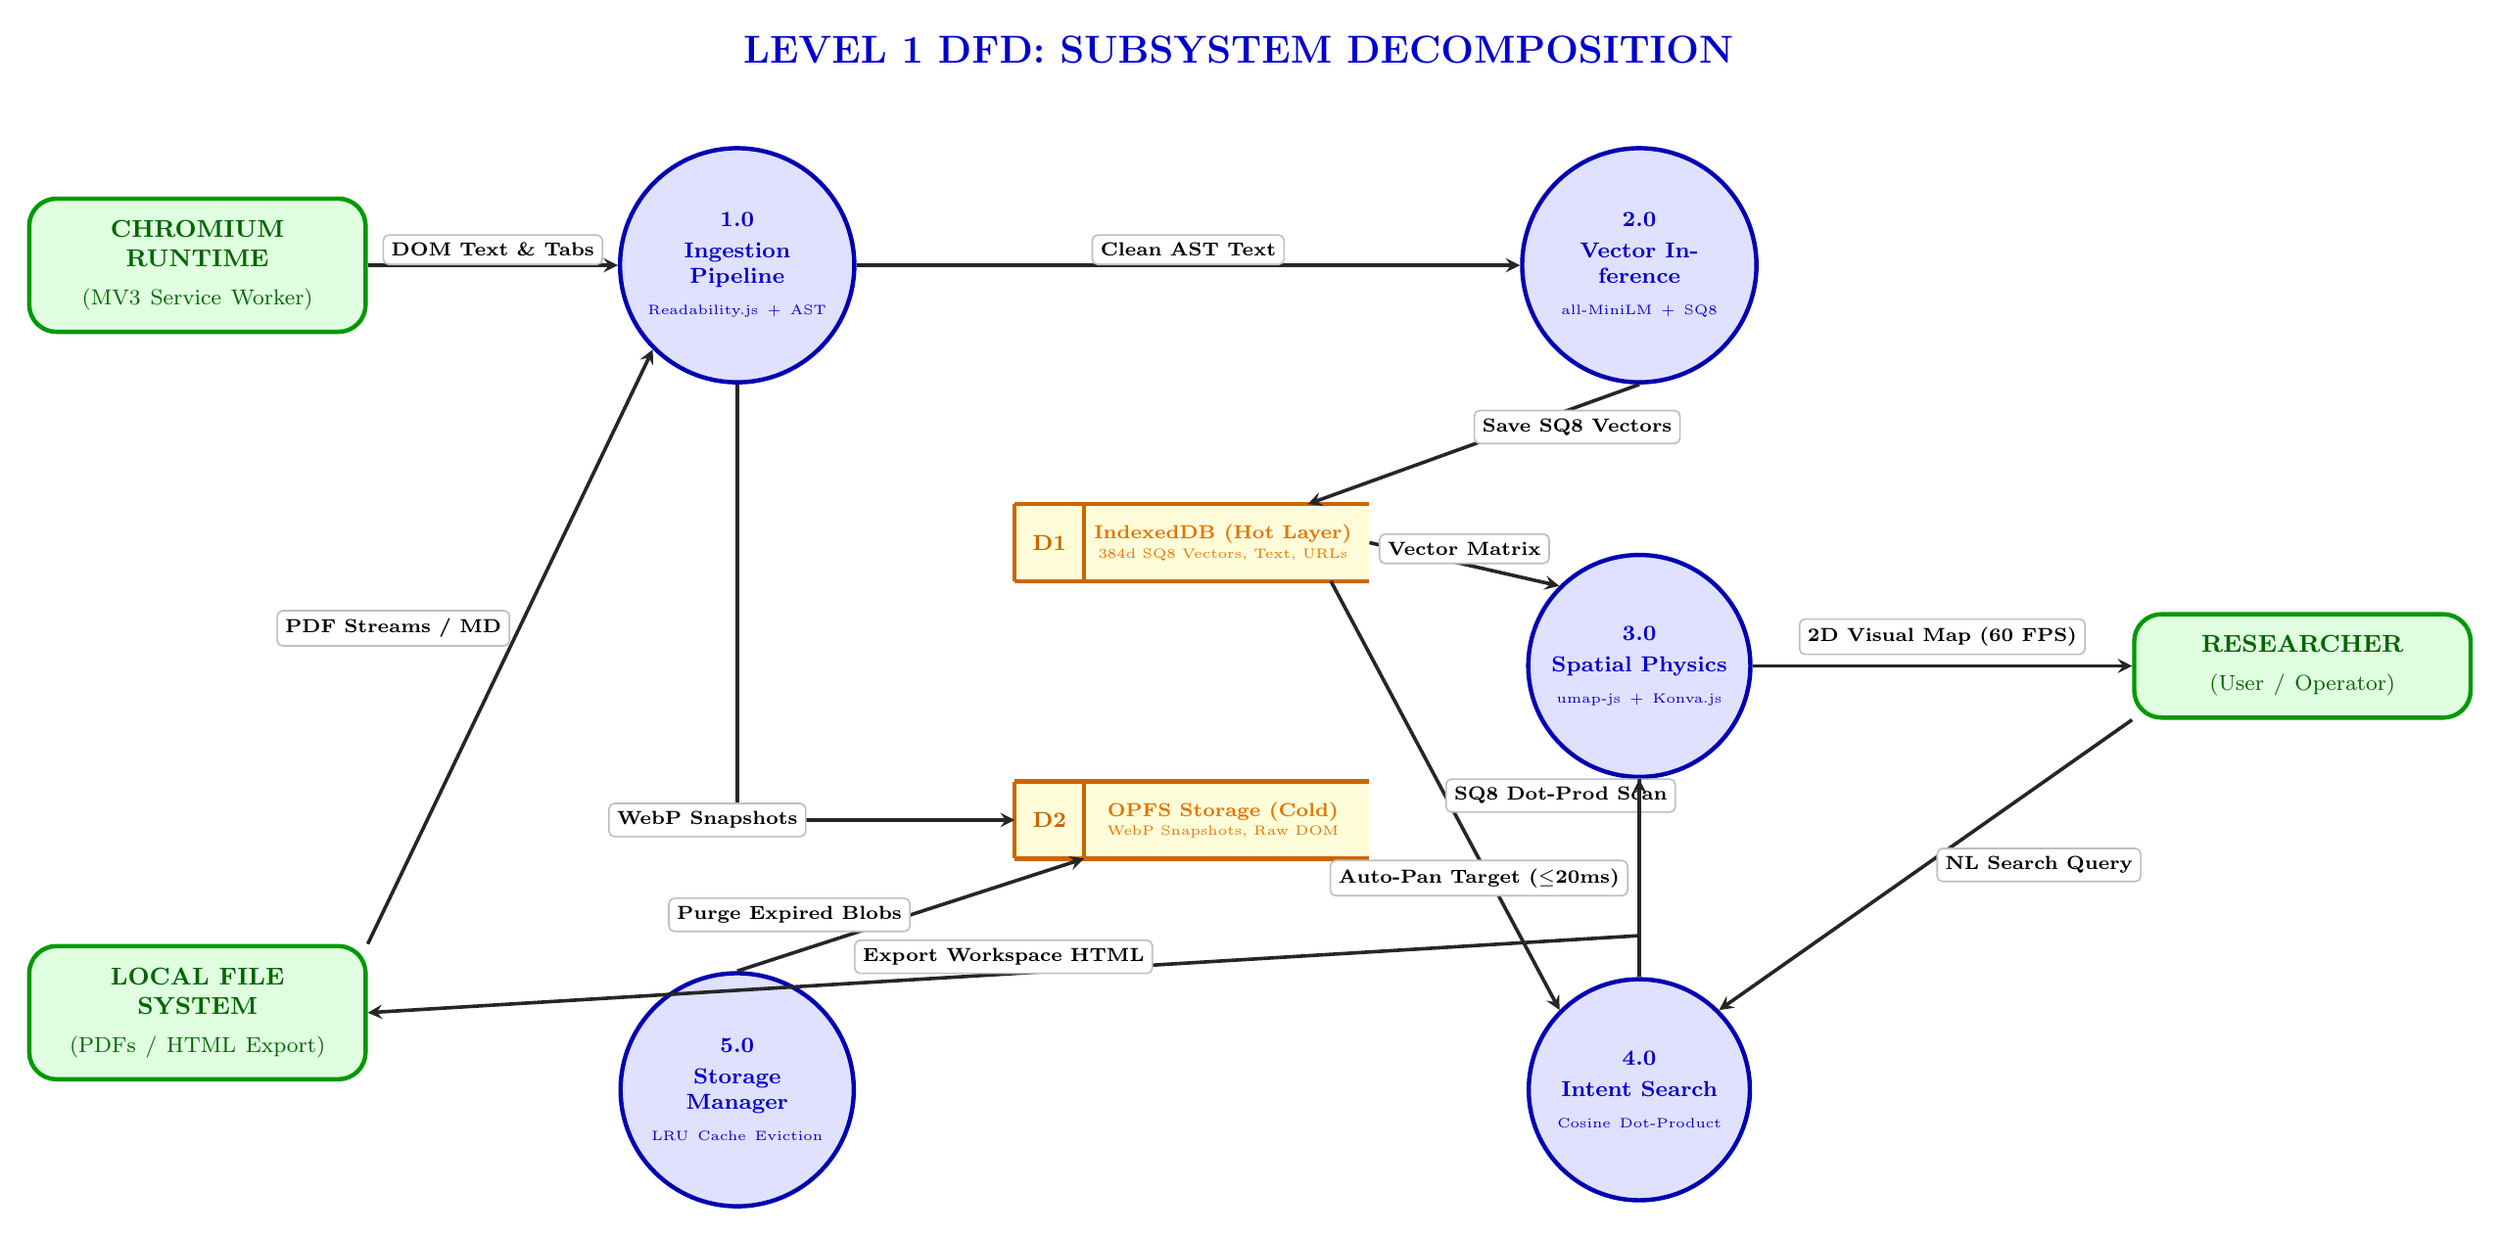
\begin{tikzpicture}[
    font=\sffamily,
    >=stealth,
    entity/.style={
        rectangle, draw=green!60!black, fill=green!12, line width=1.6pt, rounded corners=10pt,
        text width=3.8cm, align=center, inner sep=8pt, font=\small\bfseries, text=green!40!black
    },
    process/.style={
        circle, draw=blue!70!black, fill=blue!12, line width=1.6pt,
        text width=2.4cm, align=center, inner sep=3pt, font=\footnotesize\bfseries, text=blue!80!black
    },
    flow/.style={
        ->, >=stealth, line width=1.3pt, draw=black!85
    },
    labelbox/.style={
        fill=white, draw=gray!50, line width=0.6pt, rounded corners=2pt,
        inner sep=3pt, font=\scriptsize\bfseries, text=black
    }
]

    % Title
    \node[font=\Large\bfseries, text=blue!80!black] at (0, 8.0) {LEVEL 1 DFD: SUBSYSTEM DECOMPOSITION};

    % =========================================================================
    % 1. External Entities (Far Outer Bounds)
    % =========================================================================
    \node[entity] (chromium) at (-13.5, 5.2) {CHROMIUM RUNTIME\\[3pt]\footnotesize\normalfont(MV3 Service Worker)};
    \node[entity] (fs) at (-13.5, -4.5) {LOCAL FILE SYSTEM\\[3pt]\footnotesize\normalfont(PDFs / HTML Export)};
    \node[entity] (user) at (13.8, 0.0) {RESEARCHER\\[3pt]\footnotesize\normalfont(User / Operator)};

    % =========================================================================
    % 2. Circular Subsystem Processes (Huge 8.6cm Distance between 3.0 and User!)
    % =========================================================================
    \node[process] (p1) at (-6.5, 5.2) {1.0\\[2pt]Ingestion Pipeline\\[2pt]\tiny\normalfont Readability.js + AST};
    \node[process] (p2) at (5.2, 5.2) {2.0\\[2pt]Vector Inference\\[2pt]\tiny\normalfont all-MiniLM + SQ8};
    \node[process] (p3) at (5.2, 0.0) {3.0\\[2pt]Spatial Physics\\[2pt]\tiny\normalfont umap-js + Konva.js};
    \node[process] (p4) at (5.2, -5.5) {4.0\\[2pt]Intent Search\\[2pt]\tiny\normalfont Cosine Dot-Product};
    \node[process] (p5) at (-6.5, -5.5) {5.0\\[2pt]Storage Manager\\[2pt]\tiny\normalfont LRU Cache Eviction};

    % =========================================================================
    % 3. Open-Ended Data Stores (Centered)
    % =========================================================================
    % D1: IndexedDB (Hot Layer)
    \begin{scope}[shift={(-0.6, 1.6)}]
        \fill[yellow!15] (-2.3, -0.5) rectangle (2.3, 0.5);
        \draw[line width=1.6pt, draw=orange!80!black] (-2.3, 0.5) -- (2.3, 0.5);
        \draw[line width=1.6pt, draw=orange!80!black] (-2.3, -0.5) -- (2.3, -0.5);
        \draw[line width=1.6pt, draw=orange!80!black] (-2.3, -0.5) -- (-2.3, 0.5);
        \draw[line width=1.2pt, draw=orange!80!black] (-1.4, -0.5) -- (-1.4, 0.5);
        \node[font=\footnotesize\bfseries, text=orange!80!black] at (-1.85, 0) {D1};
        \node[align=center, font=\scriptsize\bfseries, text=orange!90!black] at (0.4, 0) {IndexedDB (Hot Layer)\\[-1pt]\tiny\normalfont 384d SQ8 Vectors, Text, URLs};
        \coordinate (d1_north) at (1.5, 0.5);
        \coordinate (d1_east) at (2.3, 0);
        \coordinate (d1_south_east) at (1.8, -0.5);
    \end{scope}

    % D2: OPFS Storage (Cold Layer)
    \begin{scope}[shift={(-0.6, -2.0)}]
        \fill[yellow!15] (-2.3, -0.5) rectangle (2.3, 0.5);
        \draw[line width=1.6pt, draw=orange!80!black] (-2.3, 0.5) -- (2.3, 0.5);
        \draw[line width=1.6pt, draw=orange!80!black] (-2.3, -0.5) -- (2.3, -0.5);
        \draw[line width=1.6pt, draw=orange!80!black] (-2.3, -0.5) -- (-2.3, 0.5);
        \draw[line width=1.2pt, draw=orange!80!black] (-1.4, -0.5) -- (-1.4, 0.5);
        \node[font=\footnotesize\bfseries, text=orange!80!black] at (-1.85, 0) {D2};
        \node[align=center, font=\scriptsize\bfseries, text=orange!90!black] at (0.4, 0) {OPFS Storage (Cold)\\[-1pt]\tiny\normalfont WebP Snapshots, Raw DOM};
        \coordinate (d2_west) at (-2.3, 0);
        \coordinate (d2_south_west) at (-1.4, -0.5);
    \end{scope}

    % =========================================================================
    % 4. Data Flow Connections (Generous Spacing & Zero Collisions)
    % =========================================================================
    % Chromium -> 1.0
    \draw[flow] (chromium.east) -- (p1.west) 
        node[midway, above, labelbox] {DOM Text \& Tabs};

    % Local FS -> 1.0 (PDF Ingestion)
    \draw[flow] (fs.north east) -- (p1.south west) 
        node[midway, above left, labelbox] {PDF Streams / MD};

    % 1.0 -> 2.0 (AST Text across the top)
    \draw[flow] (p1.east) -- (p2.west) 
        node[midway, above, labelbox] {Clean AST Text};

    % 2.0 -> D1 (Save SQ8 Vectors)
    \draw[flow] (p2.south) -- (d1_north) 
        node[midway, above right, labelbox] {Save SQ8 Vectors};

    % 1.0 -> D2 (Snapshots via dedicated vertical channel at x = -6.5)
    \draw[flow] (p1.south) -- (-6.5, -2.0) -- (d2_west) 
        node[near start, left, labelbox] {WebP Snapshots};

    % D1 -> 3.0 (Vector Matrix)
    \draw[flow] (d1_east) -- (p3.north west) 
        node[midway, above, labelbox] {Vector Matrix};

    % D1 -> 4.0 (SQ8 Scan)
    \draw[flow] (d1_south_east) -- (p4.north west) 
        node[midway, right, labelbox] {SQ8 Dot-Prod Scan};

    % 4.0 -> 3.0 (Auto-Pan Target - label placed on LEFT)
    \draw[flow] (p4.north) -- (p3.south) 
        node[midway, left=4pt, labelbox] {Auto-Pan Target ($\le$20ms)};

    % 3.0 -> User (2D Map - 8.6cm wide space!)
    \draw[flow] (p3.east) -- (user.west) 
        node[midway, above=4pt, labelbox] {2D Visual Map (60 FPS)};

    % User -> 4.0 (NL Query - label placed on RIGHT)
    \draw[flow] (user.south west) -- (p4.north east) 
        node[midway, right=4pt, labelbox] {NL Search Query};

    % 5.0 -> D2 (Purge)
    \draw[flow] (p5.north) -- (d2_south_west) 
        node[midway, left, labelbox] {Purge Expired Blobs};

    % 3.0 -> Local File System (Export Workspace HTML - clean horizontal bus along y = -3.5)
    \draw[flow] (p3.south) -- (5.2, -3.5) -- (fs.east) 
        node[midway, above, labelbox] {Export Workspace HTML};

\end{tikzpicture}
}
\end{center}
\end{document}